\chapter{Methodology}

\section{Overview}

The process depicted in Figure \ref{fig:methodology_flow} is logically divided into three distinct and sequential phases: the Initialization Phase, the Federated Training Loop, and the Finalization Phase. Each phase orchestrates specific interactions between the central server, the data exchange components (including the Ethereum Blockchain and Platform Kafka), and the various client-side elements. The Initialization Phase focuses on setting up the environment and preparing the initial global model, as well as securely registering baseline model weights. Following this, the Federated Training Loop represents the iterative core of the system, where local training on client data is combined with central aggregation to collaboratively improve the global model while preserving data privacy. Finally, the Finalization Phase concludes the process by delivering the trained model and ensuring that all contributions are fairly accounted for through blockchain verification, followed by the release of resources. The subsequent sections will detail each of these phases, outlining the key actors involved and the sequence of operations.


\begin{sidewaysfigure}[htbp]
    \centering
    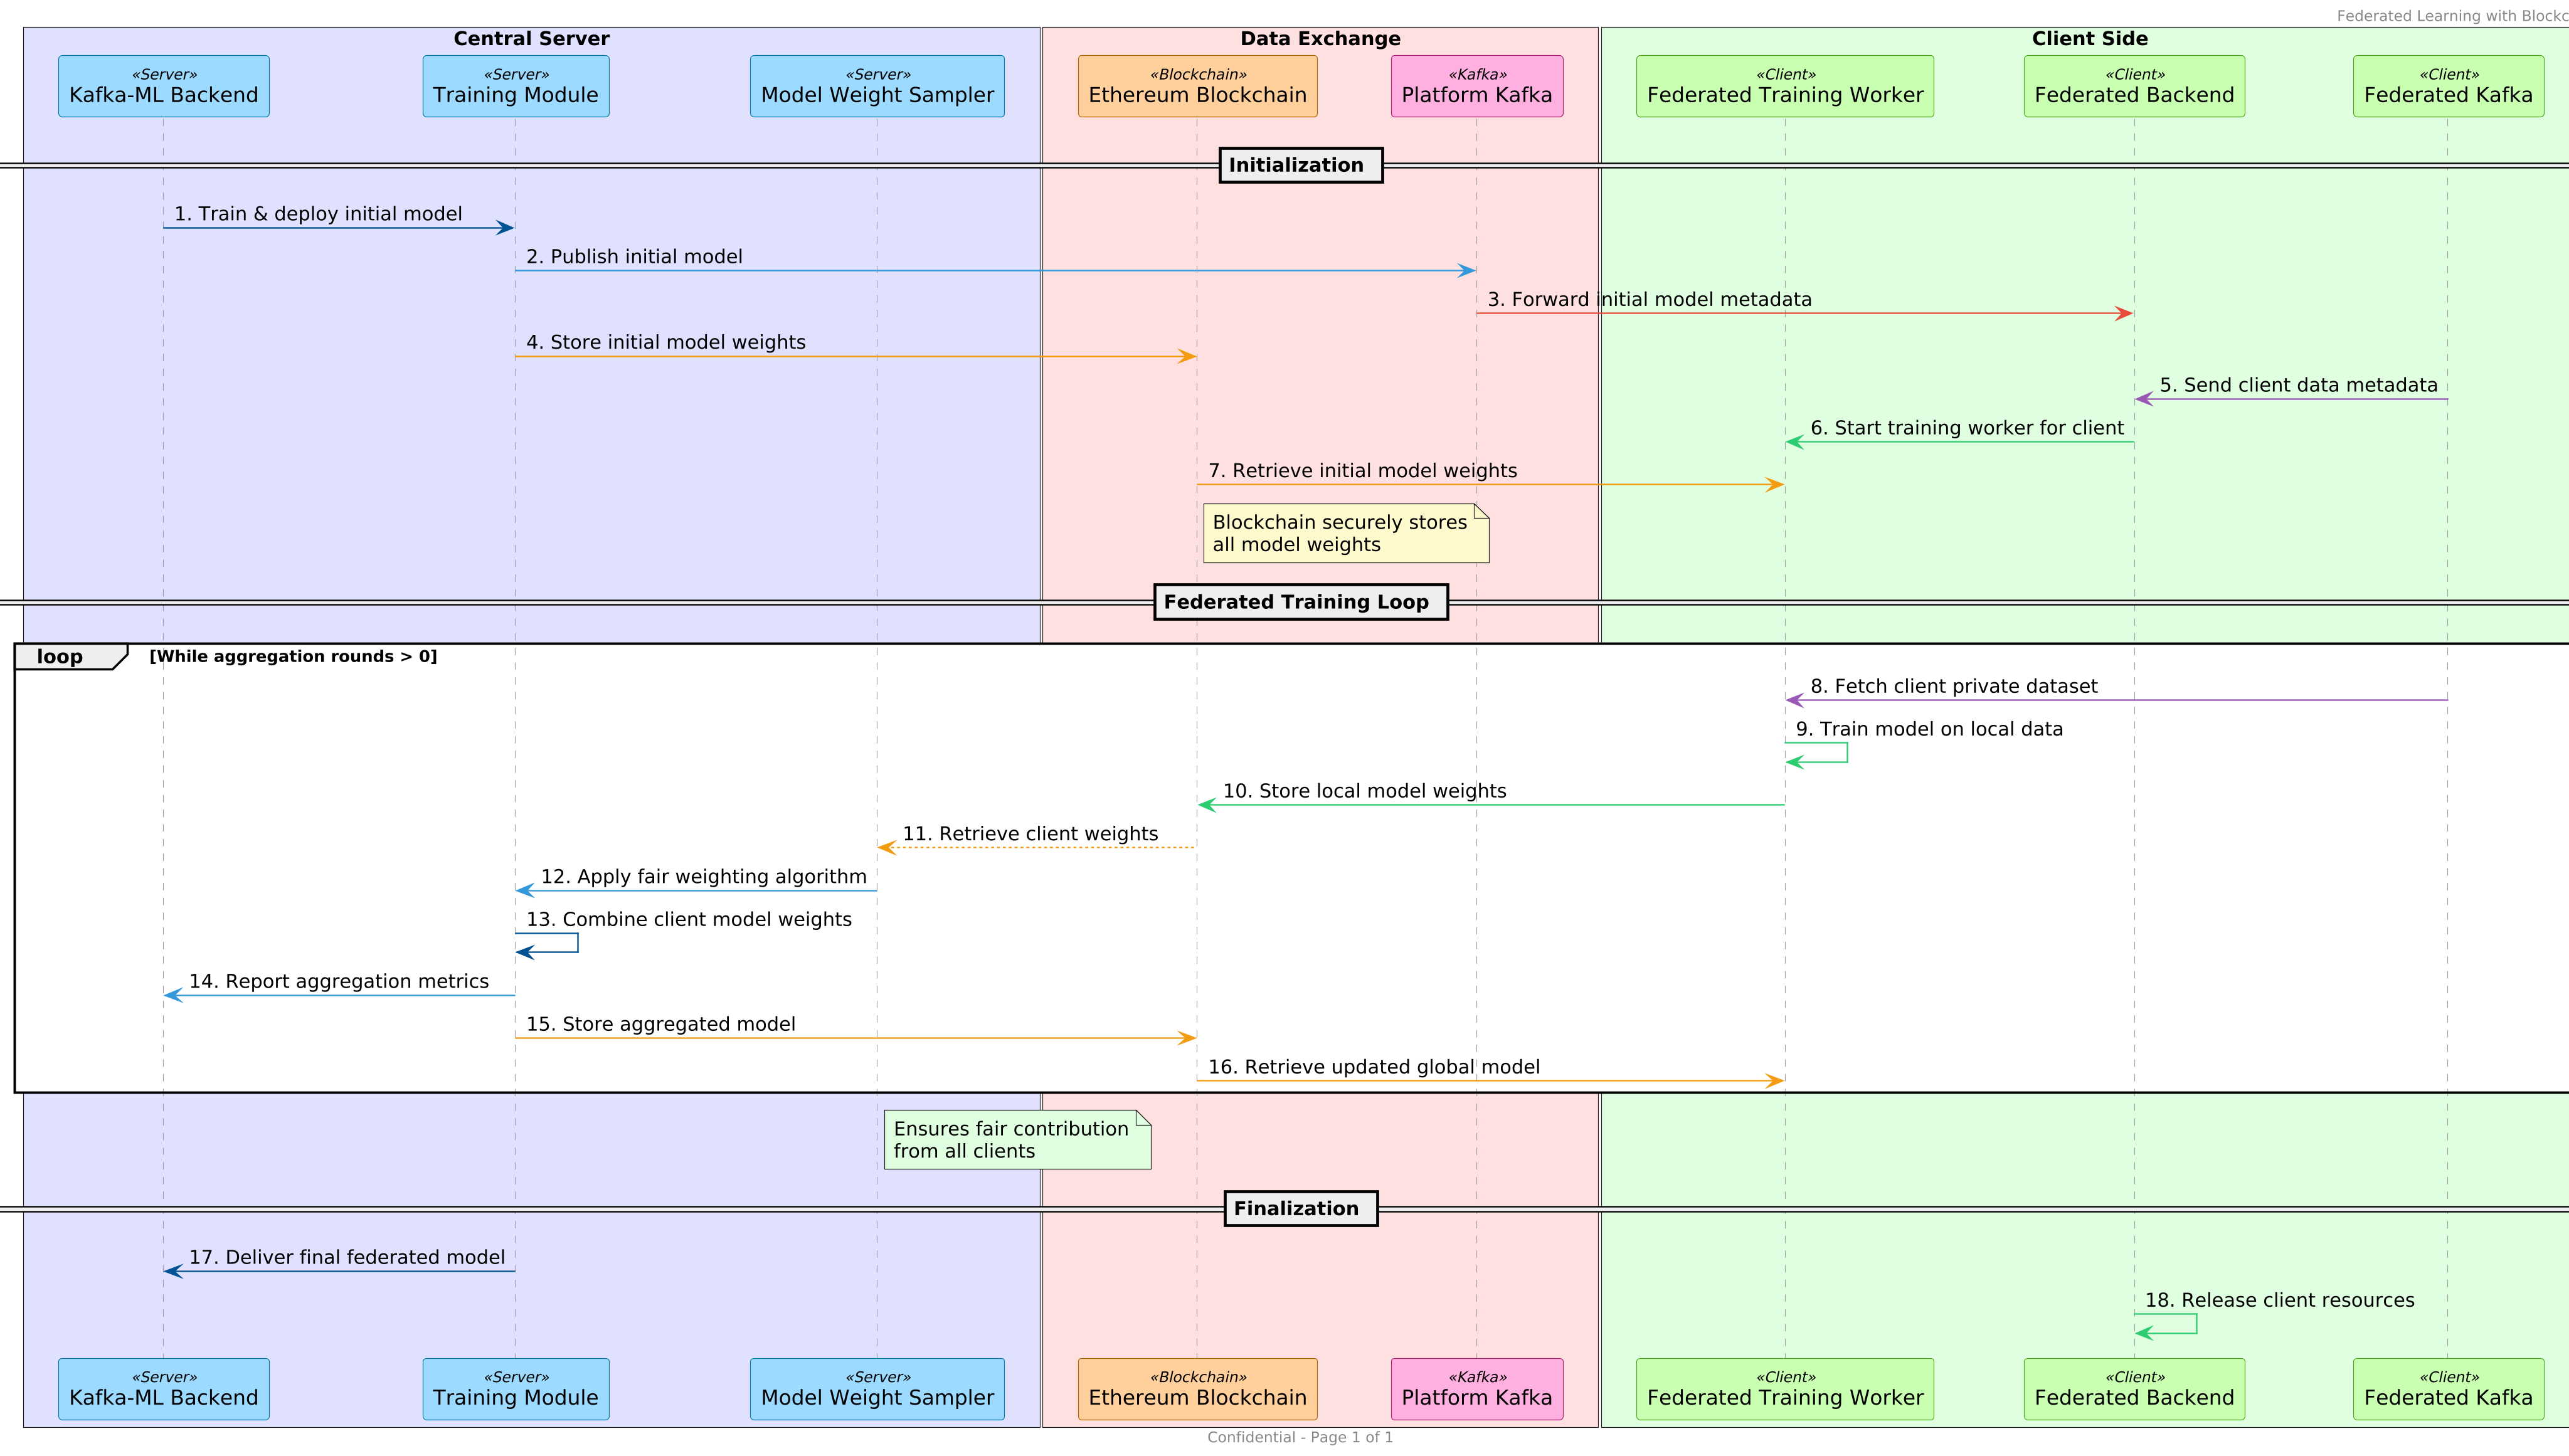
\includegraphics[scale=0.185]{MWP-Project Report Template - BD-ML-June25/methodology.png} % Include your image
    \caption{Methodology Flow Diagram}
    \label{fig:methodology_flow} % A unique label for cross-referencing this specific figure
\end{sidewaysfigure}



\section{Initialization Phase}
\label{sec:initialization_phase}

The Initialization Phase, depicted in the top block of Figure \ref{fig:methodology_flow}, focuses on setting up the environment for federated learning. Its primary objective is to prepare the initial global model, ready participating clients for training, and securely register baseline model weights.

\subsection{Key Actors and Their Roles}
\label{ssec:init_actors}
In this phase, several key entities interact:
\begin{itemize}
    \item \textbf{Central Server:} Comprising the \textit{Kafka-M. Backend}, \textit{Training Module}, and \textit{Model Weight Sampler}, it is responsible for initiating the federated learning process.
    \item \textbf{Data Exchange:} The \textit{Ethereum Blockchain} provides a secure and immutable ledger for critical information, while \textit{Platform Kafka} facilitates efficient data streaming.
    \item \textbf{Client Side:} Represented by the \textit{Federated Training Worker}, \textit{Federated Backend}, and \textit{Federated Kafka}, these components prepare to receive training tasks and contribute to the global model.
\end{itemize}

\subsection{Process Flow during Initialization}
\label{ssec:init_process}
The sequence of events in the Initialization Phase is as follows:
\begin{enumerate}
    \item \textbf{Model Deployment (Steps 1-2):} The \textit{Training Module} within the Central Server trains and deploys an initial global model. This model is then published, making it accessible for distribution.
    \item \textbf{Initial Model Weight Handling (Steps 3-4):} The \textit{Model Weight Sampler} stores these initial model weights. Subsequently, these weights are forwarded as initial model metadata towards the client side, facilitated by \textit{Platform Kafka}.
    \item \textbf{Client Preparation and Blockchain Registration (Steps 5-7):} The client's \textit{Federated Training Worker} prepares for the upcoming task by sending client data metadata. Crucially, the \textit{Ethereum Blockchain} receives and securely stores all initial model weights. This step establishes a verifiable and immutable baseline for the model's state, which is vital for ensuring integrity and transparency throughout the training process.
\end{enumerate}

\section{Federated Training Loop}
\label{sec:training_loop}

The Federated Training Loop, central to the diagram in Figure \ref{fig:methodology_flow}, represents the iterative core of the federated learning process. Its main purpose is to collaboratively improve the global model by leveraging local training on client data, while rigorously preserving data privacy. This loop is repeated until predefined convergence criteria or a maximum number of training rounds are met.

\subsection{Client-Side Training and Local Model Management}
\label{ssec:client_training}
The loop commences with client-side operations:
\begin{enumerate}
    \setcounter{enumi}{7} % Continue numbering from previous section
    \item \textbf{Fetching Private Dataset (Step 8):} Each client's \textit{Federated Training Worker} securely fetches its private dataset. It is paramount that this raw data never leaves the client device, ensuring privacy.
    \item \textbf{Local Model Training (Step 9):} The model is then trained locally on this private dataset, adapting the initial global model to the client's specific data characteristics.
    \item \textbf{Storing Local Model Weights (Step 10):} After local training, the updated model weights are stored securely on the client side.
\end{enumerate}

\subsection{Central Aggregation and Global Model Update}
\label{ssec:central_aggregation}
Following local training, the focus shifts to the central server for aggregation:
\begin{enumerate}
    \setcounter{enumi}{10} % Continue numbering
    \item \textbf{Retrieving Client Weights (Step 11):} The \textit{Training Module} within the Central Server retrieves the updated model weights from selected clients.
    \item \textbf{Applying Weighting Algorithm (Step 12):} A "fast weighting algorithm" is applied to these collected client weights. This algorithm efficiently combines the diverse contributions from individual clients.
    \item \textbf{Combining Client Model Weights (Step 13):} The client model weights are combined to form a new, aggregated model, representing a consolidated improvement from the current training round.
    \item \textbf{Reporting Aggregation Metrics (Step 14):} Relevant aggregation metrics are reported, providing insights into the progress and effectiveness of the training round.
    \item \textbf{Storing Aggregated Model (Step 15):} The newly aggregated model is stored by the Central Server.
    \item \textbf{Updating Global Model (Step 16):} This critical step involves updating the global model with the newly aggregated weights. This updated model then serves as the starting point for the subsequent iteration of the Federated Training Loop, propagating the collective intelligence back to the clients.
\end{enumerate}

\section{Finalization Phase}
\label{sec:finalization_phase}

The Finalization Phase, shown in the bottom block of Figure \ref{fig:methodology_flow}, marks the conclusion of the federated learning process. Its primary objectives are to securely deliver the collaboratively trained final model and to release the resources utilized during the process.

\subsection{Secure Model Delivery and Verification}
\label{ssec:model_delivery}
This phase begins with the delivery of the final model:
\begin{enumerate}
    \setcounter{enumi}{16} % Continue numbering
    \item \textbf{Delivering Final Federated Model (Step 17):} Once the Federated Training Loop has completed its iterations and the global model has converged or met the training criteria, the \textit{Kafka-M. Backend} of the Central Server delivers the final federated model.
\item \textbf{Blockchain for Fair Contribution:} A crucial aspect highlighted in this phase is the role of the \textit{Blockchain}. The diagram explicitly states, ``Blockchain ensures fair contribution from all clients.'' This signifies that the blockchain, having immutably recorded transactions, model updates, or participation proofs throughout the entire process, is utilized to verify the fairness and integrity of the final model. This mechanism helps to ensure that all participating clients' contributions were accurately accounted for and that the final model is trustworthy.
\end{enumerate}

\subsection{Resource Release}
\label{ssec:resource_release}
The process concludes with the release of resources:
\begin{enumerate}
    \setcounter{enumi}{17} % Continue numbering
    \item \textbf{Releasing Client Resources (Step 18):} Finally, the client-side components, specifically the \textit{Federated Backend}, release their allocated resources. This action signifies the completion of their participation in the training cycle, freeing up computational and network resources.
\end{enumerate}


